\documentclass[laporan.tex]{subfiles}

\begin{document}

\chapter{Hasil dan Pembahasan}

Data berupa foto jeruk yang telah diambil sesuai dengan langkah-langkah yang dijelaskan pada subbab \ref{photoshoot}. Pada penelitian ini dipersiapkan 12 foto dari 6 jeruk. Pada bab ini digunakan salah satu foto jeruk sebagai contoh hasil pengolahan data.

\begin{figure}[h]
\centering
\includegraphics[width=8cm]{../data/res/DSC_2996.JPG}
\caption{Foto jeruk yang diolah}
\end{figure}

\section{Pengolahan Data Awal}

Foto jeruk diperkecil resolusinya dan disunting secara manual untuk menghilangkan objek latar belakang. Hasil pengolahan awal ditunjukkan pada gambar \ref{fig:imgedited}.

\begin{figure}[h]
\centering
\includegraphics[width=8cm]{../olahdata/proc/smoothcrop/DSC_2996.png}
\caption{Gambar yang sudah dibersihkan}
\label{fig:imgedited}
\end{figure}

\section{Pengolahan Dengan Algoritma}

\subsection{\emph{Thresholding}}

\emph{Thresholding} dengan metode Otsu diterapkan pada tiap komponen warna. Nilai \emph{threshold} untuk data contoh ditampilkan di tabel \ref{table:threshval}

\begin{table}[h]
\centering
\begin{tabular}{|l|l|}
\hline
Komponen warna & Nilai \emph{Threshold} \\
\hline
R & 82 \\
G & 79 \\
B & 44 \\
\hline
\end{tabular}
\caption{Hasil \emph{threshold} metode Otsu}
\label{table:threshval}
\end{table}


\subsection{Klasifikasi \emph{Pixel} Awal}

Hasil klasifikasi awal membagi jeruk menjadi 8 kelas berdasarkan segmentasi komponen-komponen warna primer dengan metode Otsu. Pada contoh ditunjukkan visualisasi hasil klasifikasi pada gambar \ref{fig:classinit}, nilai-nilai intensitas asli \emph{pixel} digantikan dengan rata-rata intensitas kelas masing-masing \emph{pixel} tersebut. Tabel rata-rata intensitas \ref{table:clsrgbavg1} menunjukkan bahwa seluruh kelas warna muncul pada citra yang diuji.

\begin{figure}[h]
\centering
\includegraphics[width=8cm]{../olahdata/proc/data/seg3a.png}
\caption{Visualisasi hasil klasifikasi \emph{pixel} awal}
\label{fig:classinit}
\end{figure}

\begin{table}[h]
\centering
\begin{tabular}{|l|l|l|l|}
\cline{1-4}
\multirow{2}{*}{Kelas} & \multicolumn{3}{l|}{Rata-rata intensitas} \\
\cline{2-4}
 & R & G & B \\
\cline{1-4}
1 & 1.67 & 0.72 & 0.75 \\
2 & 61.11 & 68.35 & 51.13 \\
3 & 76.11 & 82.57 & 21.15 \\
4 & 73.85 & 87.14 & 57.80 \\
5 & 84.01 & 76.80 & 25.06 \\
6 & 82.90 & 77.18 & 49.90 \\
7 & 160.50 & 154.17 & 11.82 \\
8 & 180.61 & 177.75 & 85.59 \\
\cline{1-4}
\end{tabular}
\caption{Nilai rata-rata intensitas tiap kelas}
\label{table:clsrgbavg1}
\end{table}

\subsubsection{Pembuatan Kelas Baru}

Kelas-kelas \emph{pixel} selanjutnya disusun ulang berdasarkan jarak antarkelas yang dihitung dari \emph{mean squared distance} rata-rata intensitas. Kelas yang saling bertetangga digabungkan kemudian rata-rata intensitas baru dihitung untuk tiap kelas. Tabel \ref{table:clsdist} menunjukkan hasil perhitungan jarak antarkelas untuk data contoh, tabel \ref{table:newclass} menunjukkan kelas baru yang dibuat. Tabel \ref{table:newclassavg} memuat rata-rata intensitas kelas baru.


\begin{table}[h]
\centering
\begin{tabular}{|l|l|l|l|l|l|l|l|l|}
\hline
Kelas & K1 & K2 & K3 & K4 & K5 & K6 & K7 & K8 \\
\hline
K1 & -- & 59.20 & 64.79 & 72.49 & 65.85 & 70.03 & 127.27 & 153.05 \\
K2 & 59.20 & -- & 21.18 & 13.66 & 20.62 & 13.60 & 79.14 & 95.68 \\
K3 & 64.79 & 21.18 & --	& 21.39 & 5.80 & 17.26 & 63.84 & 89.52 \\
K4 & 72.49 & 13.66 & 21.39 & --	& 20.67 & 9.01 & 68.59 & 82.46 \\
K5 & 65.85 & 20.62 & 5.80 & 20.67 & -- & 14.36 & 63.28 & 88.00 \\
K6 & 70.03 & 13.60 & 17.26 & 9.01 & 14.36 & -- & 66.83 & 83.59 \\
K7 & 127.27 & 79.14 & 63.84 & 68.59 & 63.28 & 66.83 & -- & 46.39 \\
K8 & 153.05 & 95.68 & 89.52 & 82.46 & 88.00 & 83.59 & 46.39 & -- \\
\hline
\end{tabular}
\caption{Jarak antarkelas}
\label{table:clsdist}
\end{table}

\begin{table}[h]
\centering
\begin{tabular}{|l|l|l|}
\hline
Kelas & Kelas Terdekat & Kelas Baru \\
\hline
K1 & K2 & K1 \\
K2 & K6 & K2 \\
K3 & K5 & K3 = K3 + K5 \\
K4 & K6 & K4 = K4 + K6 \\
K5 & K3 & -- \\
K6 & K4 & -- \\
K7 & K8 & K5 = K7 + K8 \\
K8 & K7 & -- \\
\hline
\end{tabular}
\caption{Penggabungan kelas}
\label{table:newclass}
\end{table}

\begin{table}[h]
\centering
\begin{tabular}{|l|l|l|l|}
\cline{1-4}
\multirow{2}{*}{Kelas} & \multicolumn{3}{l|}{Rata-rata intensitas} \\
\cline{2-4}
 & R & G & B \\
\cline{1-4}
1 & 1.67 & 1.72 & 0.75 \\
2 & 61.11 & 68.35 & 51.13 \\
3 & 78.62 & 81.10 & 22.14 \\
4 & 74.50 & 86.43 & 57.24 \\
5 & 163.00 & 157.10 & 21.04 \\
\cline{1-4}
\end{tabular}
\caption{Rata-rata intensitas kelas baru}
\label{table:newclassavg}
\end{table}

\subsubsection{Reklasifikasi \emph{Pixel}}

\emph{Pixel} pada citra asli diklasifikasi ulang berdasarkan jarak terdekat dari nilai rata-rata intensitas dengan perhitungan \emph{sum squared distance}. Gambar \ref{fig:classfinimg} menunjukkan hasil klasifikasi ulang, nilai intensitas asli tiap \emph{pixel} diganti dengan rata-rata intensitas kelas.

\begin{figure}[h]
\centering
\includegraphics[width=8cm]{../olahdata/proc/data/seg3b.png}
\caption{Hasil klasifikasi ulang \emph{pixel}}
\label{fig:classfinimg}
\end{figure}

\subsection{Operasi Morfologi}

Dari matriks data klasifikasi diambil titik-titik \emph{pixel} dengan kelas tertinggi sebagai sebuah citra biner yang menunjukkan bagian teksur normal. Operasi morfologi penutupan lubang dilakukan atas citra biner ini lalu diambil selisihnya untuk mendeteksi bagian-bagian cacat.

\begin{figure}[h]
\centering
\includegraphics[width=4cm]{../olahdata/proc/data/mask3normal.png}
\caption{\emph{Mask} yang menunjukkan tekstur normal}
\end{figure}

\begin{figure}[h]
\centering
\includegraphics[width=4cm]{../olahdata/proc/data/mask3filled.png}
\caption{Hasil penutupan lubang pada \emph{mask}}
\end{figure}

\begin{figure}[h]
\centering
\includegraphics[width=4cm]{../olahdata/proc/data/mask3blemish.png}
\caption{Daerah cacat yang dideteksi}
\end{figure}

\section{Perhitungan Luas Cacat dan Akurasi}

Sebagai acuan akurasi deteksi, digunakan citra biner cacat tekstur kulit yang digambar secara manual dengan menggunakan perangkat \emph{fuzzy select} dan \emph{color select} pada aplikasi pengolah citra Gimp. Prosentase hasil deteksi dan akurasi ditunjukkan pada tabel di bawah.

\begin{figure}[h]
\centering
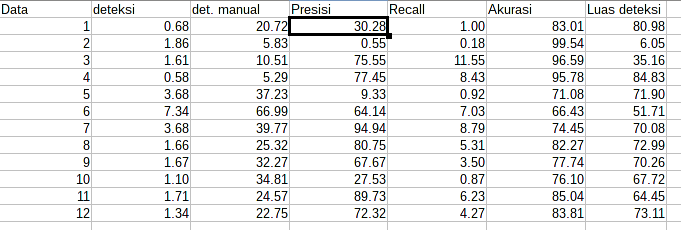
\includegraphics[width=10cm]{tex/comparison.png}
\caption{Akurasi deteksi}
\end{figure}
%\begin{tabular}{|l|l|l|l|l|l|l|}
%\hline
%Berkas citra & \% deteksi otomatis & \% deteksi manual & Presisi & \emph{Recall} & Akurasi & \% luas yang diproses \\
%\hline
%\hline
%\end{tabular}

\section{Interpretasi Hasil}

Data menunjukkan bahwa metode deteksi menghasilkan hasil yang bervariasi, dengan akurasi tinggi, presisi yang cukup baik, namun \emph{recall} sangat rendah. Tingkat \emph{recall} yang rendah ini disebabkan karena hanya sebagian dari permukaan jeruk yang dapat dideteksi, dan terutama karena citra biner yang digunakan untuk referensi kurang akurat.

Metode ini selain tidak dirancang untuk mendeteksi cacat pada bagian-bagian gelap pada tepi jeruk, juga tidak dapat mendeteksi cacat pada bagian tengah jeruk yang berkilap karena sorotan sumber cahaya. Perlu dilakukan penyesuaian pencahayaan untuk mengurangi atau menghindari munculnya kilap di tengah objek.

%Karena metode yang digunakan mengacu pada tepi daerah cacat maka akurasi metode tidak diukur dari prosentase kesalahan luas cacat yang terdeteksi namun dari banyaknya daerah-daerah cacat yang terdeteksi dan ketepatan lokasi deteksi tersebut.

%(confusion matrix, presisi, akurasi)

\end{document}
